%%%%%%%%%%%%%%%%%%%%%%% file template.tex %%%%%%%%%%%%%%%%%%%%%%%%%
%
% This is a general template file for the LaTeX package SVJour3
% for Springer journals.          Springer Heidelberg 2010/09/16
%
% Copy it to a new file with a new name and use it as the basis
% for your article. Delete % signs as needed.
%
% This template includes a few options for different layouts and
% content for various journals. Please consult a previous issue of
% your journal as needed.
%
%%%%%%%%%%%%%%%%%%%%%%%%%%%%%%%%%%%%%%%%%%%%%%%%%%%%%%%%%%%%%%%%%%%
%
% First comes an example EPS file -- just ignore it and
% proceed on the \documentclass line
% your LaTeX will extract the file if required
\begin{filecontents*}{example.eps}
%!PS-Adobe-3.0 EPSF-3.0
%%BoundingBox: 19 19 221 221
%%CreationDate: Mon Sep 29 1997
%%Creator: programmed by hand (JK)
%%EndComments
gsave
newpath
  20 20 moveto
  20 220 lineto
  220 220 lineto
  220 20 lineto
closepath
2 setlinewidth
gsave
  .4 setgray fill
grestore
stroke
grestore
\end{filecontents*}
%
\RequirePackage{fix-cm}
%
%\documentclass{svjour3}                     % onecolumn (standard format)
%\documentclass[smallcondensed]{svjour3}     % onecolumn (ditto)
\documentclass[smallextended]{svjour3}       % onecolumn (second format)
%\documentclass[twocolumn]{svjour3}          % twocolumn
%
\smartqed  % flush right qed marks, e.g. at end of proof
%
\usepackage{graphicx}
%
% \usepackage{mathptmx}      % use Times fonts if available on your TeX system
%
% insert here the call for the packages your document requires
%\usepackage{latexsym}
% etc.
%
% please place your own definitions here and don't use \def but
% \newcommand{}{}
%
% Insert the name of "your journal" with
% \journalname{myjournal}
%
\begin{document}

\title{Using Citation Data to Study Computer Science%\thanks{Grants or other notes
%about the article that should go on the front page should be
%placed here. General acknowledgments should be placed at the end of the article.}
}
\subtitle{Relationship With Other Fields}

%\titlerunning{Short form of title}        % if too long for running head

\author{Sitaram Devarakonda  \and
        Dmitriy Korobskiy \and
        Tandy Warnow \and
        George Chacko }

%\authorrunning{Short form of author list} % if too long for running head

\institute{Sitaram Devarakonda,  \at
              Netelabs, NET ESolutions Corporation, McLean, VA \\
              %Tel.: +123-45-678910\\
              %Fax: +123-45-678910\\
              \email{sitaram@nete.com}           %  \\
%             \emph{Present address:} of F. Author  %  if needed
           \and
	  Dmitriy Korobskiy \at
              Netelabs, NET ESolutions Corporation, McLean, VA \\
              \email{dk@nete.com}
                  \and
           Tandy Warnow \at
              Dept of Computer Science, University of Iliinois Urbana-Champaign, Champaign IL \\
              \email{warnow@illinois.edu}
                  \and
           George Chacko \at
              Netelabs, NET ESolutions Corporation, McLean, VA \\
              \email{netelabs@nete.com}
}

\date{Received: date / Accepted: date}
% The correct dates will be entered by the editor


\maketitle

\begin{abstract}
Computer science and its applications has experienced dramatic growth and diversification over the last twenty years. Towards understanding the nature of these changes, we analyze a cohort of the computer science literature using a historiographic approach. To understand the features of this cohort and the flow of information within its components, we construct article level clusters whose elements are linked by citations or co-citations, and reconcile them with subject categories in the Scopus database. 

\keywords{Bibliometrics \and Clustering \and Knowledge Evolution \and Research Evaluation}
% \PACS{PACS code1 \and PACS code2 \and more}
\subclass{01A85 \and 01A90} %\and more}
\end{abstract}

\section{Introduction}
\label{intro}

Cite Alan Porter on expanding universe versus myopic focus. Cite Traag, Waltman, Lariviere papers. Peter Sjögårde and Per Ahlgren, Loet Leydesdorff, Caroline S. Wagner and Lutz Bornmann, Discontinuities in citation relations among journals: self-organized criticality as a model of scientific revolutions and change, Scientometrics, 10.1007/s11192-018-2734-6, 116, 1, (623-644), (2018). Antonio Perianes-Rodriguez and Javier Ruiz-Castillo, A comparison of the Web of Science and publication-level classification systems of science, Journal of Informetrics, 10.1016/j.joi.2016.10.007, 11, 1, (32-45), (2017). Qi Wang and Ludo Waltman, Large-scale analysis of the accuracy of the journal classification systems of Web of Science and Scopus, Journal of Informetrics, 10.1016/j.joi.2016.02.003, 10, 2, (347-364), (2016). Henry Small, Kevin W. Boyack and Richard Klavans, Identifying emerging topics in science and technology, 
Crossref

%%%%%%%%%%%%%%%
\section{Materials and Methods}


\emph{Data} The dblp computer science bibliography consisting of 7,079,994 records was downloaded as dblp-2018-08-01.xml.gz from  `https://dblp.uni-trier.de/xml/`. Publications were parsed from the xml source file and loaded into a PostgreSQL database. These parsed records were then matched to Scopus identifiers using PostgreSQL's full text search feature applied to document titles. The process involves parsing Scopus document titles into tokens, reducing the tokens into lexemes and returning a ts\_vector which lists the lexemes together with their positions. The ts\_vector is then matched with DBLP document titles. A ts\_rank is returned based on the frequency of matching lexemes. Only records in dblp with DOIs (4,291,130) were considered and only matches with a rank of $>$ 0.99 were accepted. This procedure resulted in a dataset of 634,100 publications. Cited references for these were extracted from Scopus, resulting in a total of 3,960,503 nodes (publications and references) and 11,992,387 edges that represents citations of these references and publications within the dataset. This dataset was labelled \emph{comp}.\par \emph{Clustering by Direct Citation} Graclus software was downloaded from \\`http://www.cs.utexas.edu/users/dml/Software/graclus.html'. The \emph{comp} dataset was cast as an undirected graph and stored in a file with a header line indicating the number of nodes and edges. Graclus accepts the number of clusters required as a parameter, so we used 10,15, 20, 25, 30, 40, and 50 as this parameter and  \emph{comp} as input. Based on criteria articulated in the Louvain and Leiden clustering algorithms, we chose 20 clusters as the number of output clusters. \par \emph{Clustering by Co-Citation} To build clusters using co-citations, we slightly modified the approach of Small and Sweeney (1985) as follows. We first calculated the number of citations accumulated across Scopus for all 634,100 articles in \emph{comp}. After discarding those publications that had not been cited at all, we restricted further analysis to the those in the 90th percentile or higher resulting in a dataset of size 50,869. We then identified 897,407 publications in Scopus that cite the 50,869 previously selected papers from \emph{comp}. The cited references in these papers were restricted to those in the set of 50,869 highly cited papers previously identified. For each publication in turn, all possible reference pairs were generated. The frequency of these co-cited pairs was then computed across the dataset  and normalized using Salton's cosine formula~\cite{salton_citation_1979}. A total of 2,208,135 unique co-cited pairs were thus obtained. These data were represented in an edge list where each node was a publication and the weighted edge between the pair was the normalized co-citation frequency. Variable level clustering involves iteratively selecting the edges with the highest normalized co-citation value and extracting connected components from the graph. 
\begin{figure}[ht]
% Use the relevant command to insert your figure file.
% For example, with the graphicx package use
  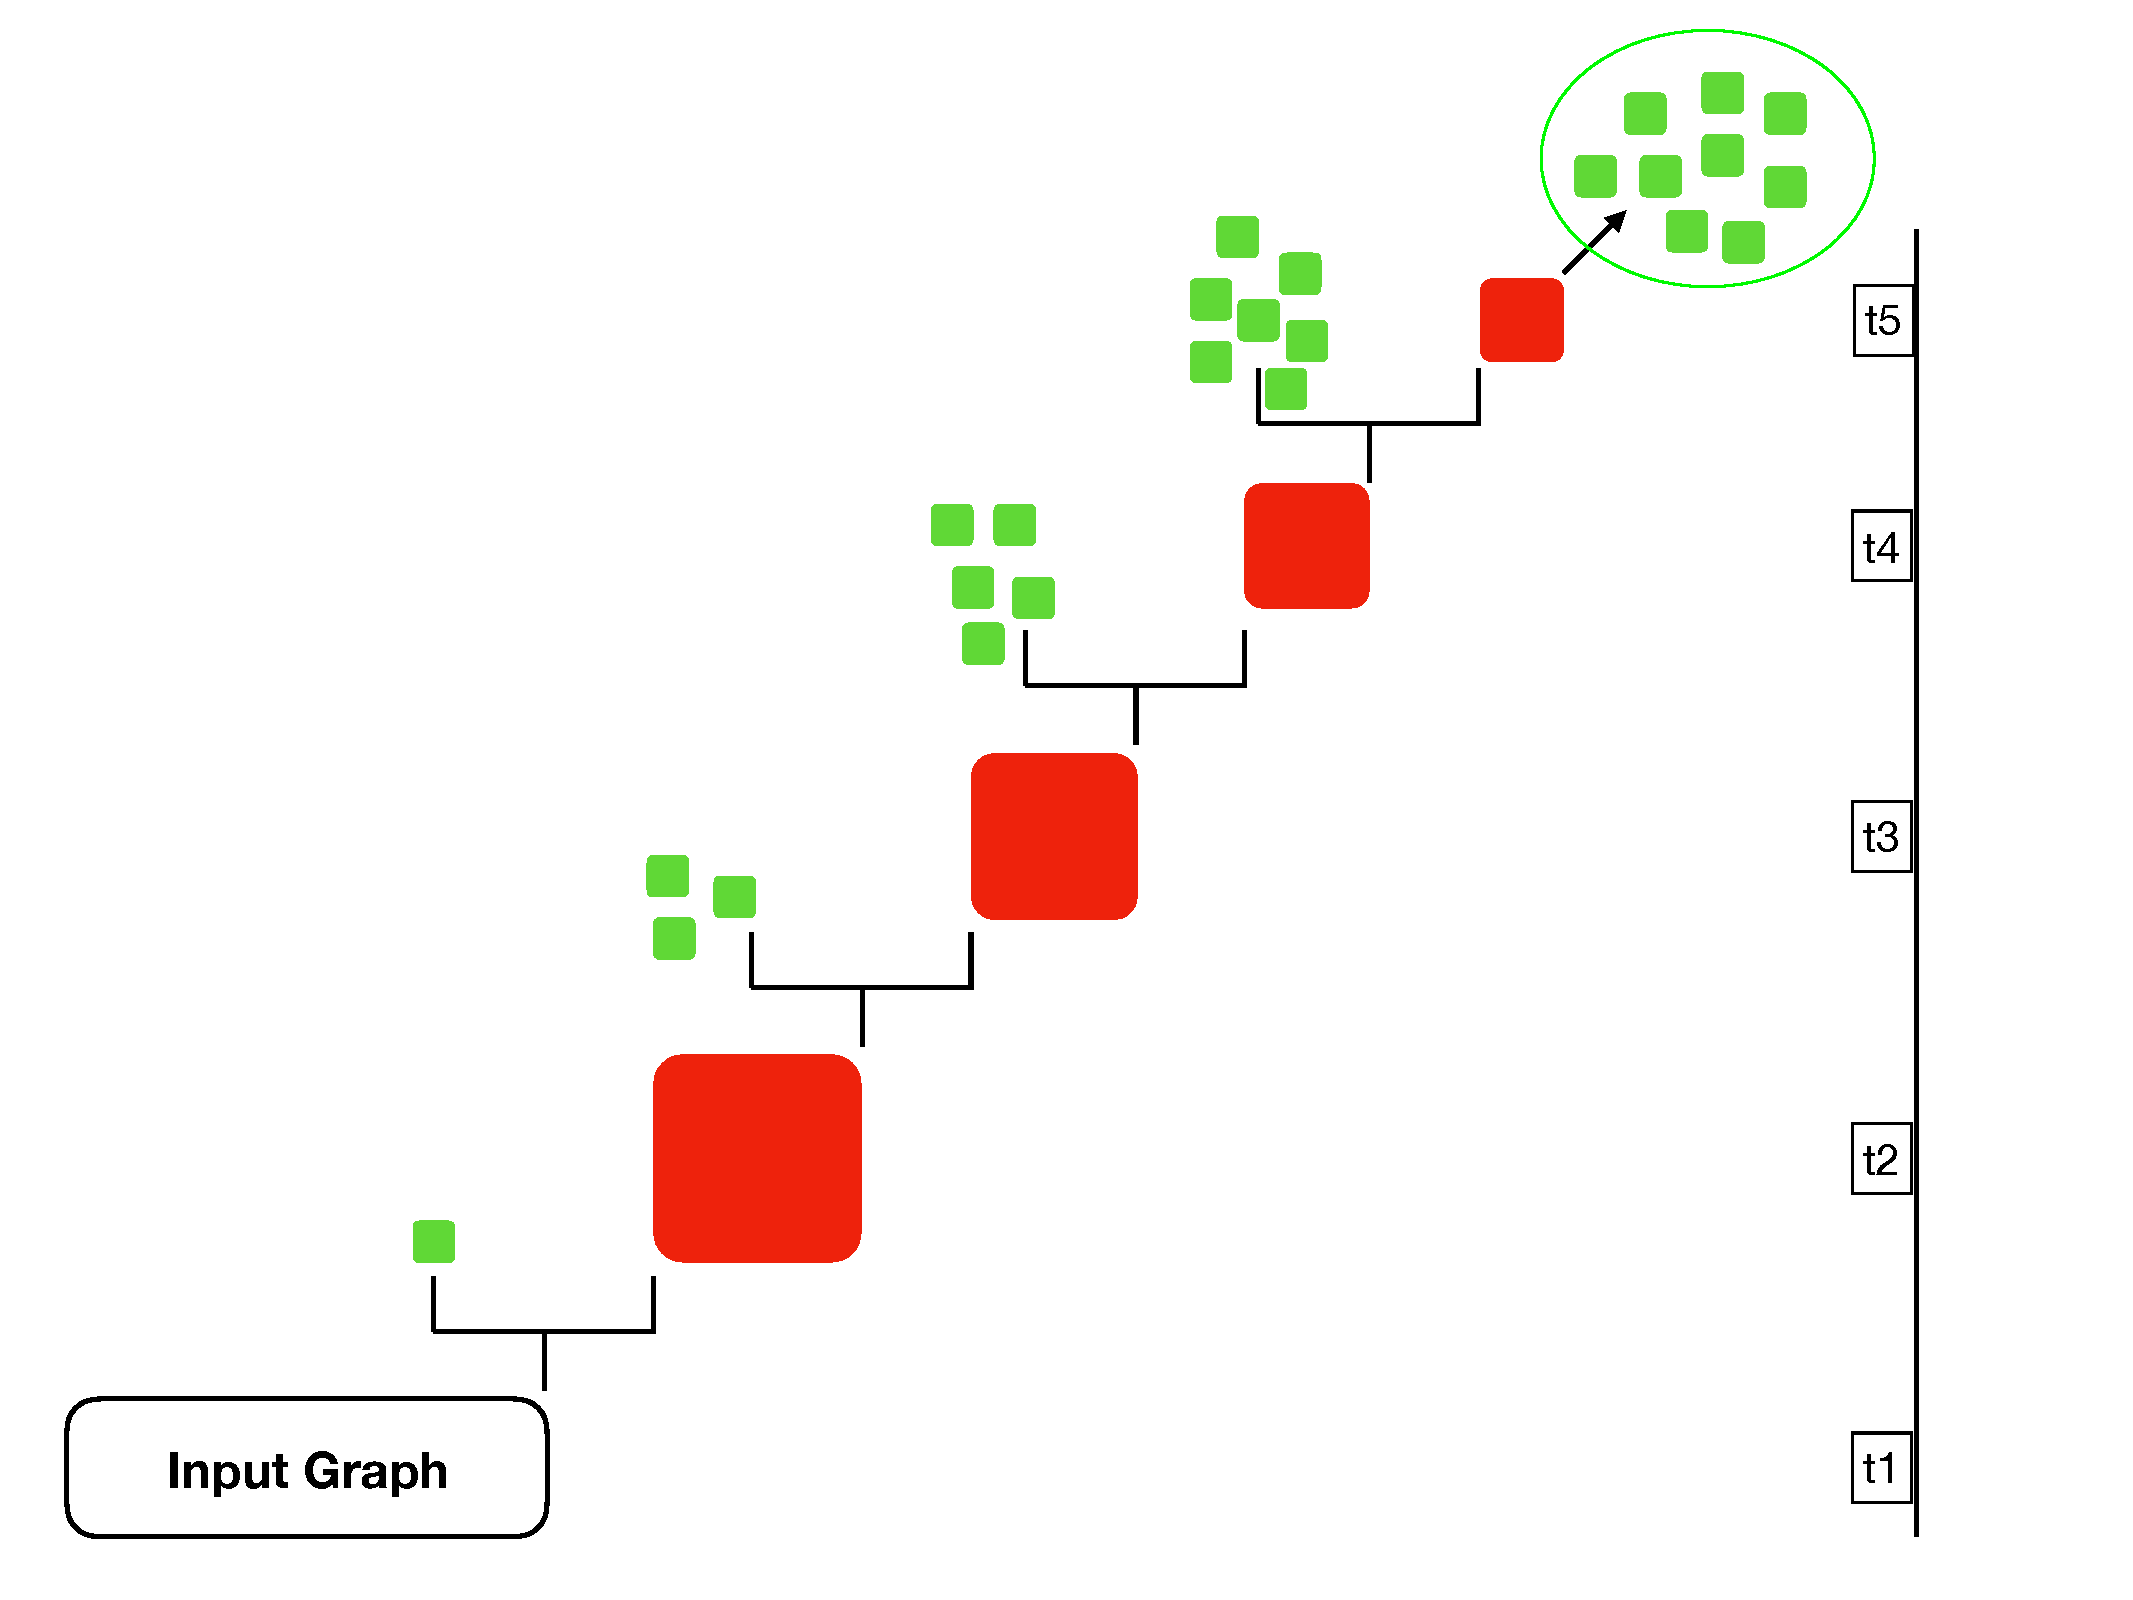
\includegraphics[scale=0.3]{vlc.pdf}
% figure caption is below the figure
\caption{Schematic representation of variable clustering protocol modified from Small and Sweeney (1985). Three parameters are specified (i) a threshold or starting level based on a quantile of normalized co-citation frequency (ii) a level increment (iii) a maximum cluster size. Input data is a set of co-cited publications with edge-weight defined by normalized co-citation frequencies. Green clusters are within the max cluster size. At the initial threshold, $t1$, a single cluster below the maximum cluster size, $mcs$ (green), along with one large cluster above it (red) are generated. As the threshold is incremented to $t2$, additional clusters of acceptable size is generated. The cascade continues to completion, which is defined by all clusters being of size less than or equal to the $mcs$. In this schematic, five rounds are adequate.}
\label{vlc_process}       % Give a unique label
\end{figure}

An issue faced is the generation of very large clusters by chaining through low edge weights. To address this, we used Small and Sweeney's variable clustering approach~\cite{small_clustering_1985} with initial parameters of threshold ($t$) = 0.5 (median normalized co-citation frequency), increment $i = 0.1$, and maximum cluster size, $mcs = 100$. Thus, at start, all edges below the median normalized co-citation frequency are dissolved. Clusters were formed by assembling connected components from each co-cited pair beginning with the heaviest edge weight. Clusters below size 100 were retained and any cluster larger than 200 nodes was carried over to the next round. The threshold, $t$, was then incremented by 0.1 and the process repeated while progressively incrementing $t$.  We used a bi-phasic approach where in which $t$ ranged from 0.5-0.9, after which $i$ was reduced to 0.01 for the range $0.9 <= t <= 0.99$. A final threshold of $t$=0.999 was applied to break the single remaining large cluster. All clusters generated thus, contained  less than 100 nodes.  Using this approach, 6,822 clusters containing 35,485 nodes were generated. Clusters containing only 2 nodes were then discarded bringing the total number of clusters down to 3,851. Pairwise clustering was then performed on these clusters to generate super-clusters. After 9 rounds of pairwise clustering, 12 clusters were generated resulting from agglomeration of the original 3,851 clusters 

\label{sec:1}
Text with citations \cite{RefB} and \cite{RefJ}.

\section{Results}
\label{sec:2}

Overall strategy:

\begin{itemize}
\item Spectral clustering
\begin{enumerate}
\item Subset Scopus by COMP
\item Match COMP to dblp at high stringency -> reduced number of scps
 \item Harvest cited references  from Scopus
 \item Cluster articles by direct citation using Graclus to a number that meets simple optimality criteria and does not impose cognitive challenges
 \item Reconcile cluster contents to journal classification for the purpose of referencing
 \item Infer inter-cluster relationships using direct citations, co-citations, and bibliographic coupling
\end{enumerate}
\item Co-citation based clustering
\begin{enumerate}
\item Stratify by year after subsetting by COMP and restricting to article and cp only
\item Apply fractional citation counting and identify highly-cited papers
\item Calculate normalized co-citations
\item Cluster by variable clustering method of Small
\item Evaluate major co-cited pairs
\end{enumerate}
\end{itemize}


Text with citations \cite{RefB} and \cite{RefJ}.

\subsection{Subsection title}
\label{sec:2}
as required. Don't forget to give each section
and subsection a unique label (see Sect.~\ref{sec:1}).
\paragraph{Paragraph headings} Use paragraph headings as needed.
\begin{equation}
a^2+b^2=c^2
\end{equation}

% For one-column wide figures use
\begin{figure}
% Use the relevant command to insert your figure file.
% For example, with the graphicx package use
  \includegraphics{example.eps}
% figure caption is below the figure
\caption{Please write your figure caption here}
\label{fig:1}       % Give a unique label
\end{figure}
%
% For two-column wide figures use
\begin{figure*}
% Use the relevant command to insert your figure file.
% For example, with the graphicx package use
  \includegraphics[width=0.75\textwidth]{example.eps}
% figure caption is below the figure
\caption{Please write your figure caption here}
\label{fig:2}       % Give a unique label
\end{figure*}
%
% For tables use
\begin{table}
% table caption is above the table
\caption{Please write your table caption here}
\label{tab:1}       % Give a unique label
% For LaTeX tables use
\begin{tabular}{lll}
\hline\noalign{\smallskip}
first & second & third  \\
\noalign{\smallskip}\hline\noalign{\smallskip}
number & number & number \\
number & number & number \\
\noalign{\smallskip}\hline
\end{tabular}
\end{table}


%\begin{acknowledgements}
%If you'd like to thank anyone, place your comments here
%and remove the percent signs.
%\end{acknowledgements}


% Authors must disclose all relationships or interests that 
% could have direct or potential influence or impart bias on 
% the work: 
%
% \section*{Conflict of interest}
%
% The authors declare that they have no conflict of interest.


% BibTeX users please use one of
%\bibliographystyle{spbasic}      % basic style, author-year citations
\bibliographystyle{spmpsci}      % mathematics and physical sciences
%\bibliographystyle{spphys}       % APS-like style for physics
\bibliography{comp}   % name your BibTeX data base

% Non-BibTeX users please use
\begin{thebibliography}{}
%
% and use \bibitem to create references. Consult the Instructions
% for authors for reference list style.
%
\bibitem{RefJ}
% Format for Journal Reference
Author, Article title, Journal, Volume, page numbers (year)
% Format for books
\bibitem{RefB}
Author, Book title, page numbers. Publisher, place (year)
% etc
\end{thebibliography}

\end{document}
% end of file template.tex

